\chapter{FlightGear仿真效果}\label{forward}

本章主要介绍FLightGear仿真效果,首先,是介绍FlightGear驱动飞行器模拟的步骤;然后,是介绍FlightGear系统实施的软硬件环境;最后,是展示四旋翼飞行仿真效果。
\section{FlightGear飞行模拟器驱动}
FlightGear实现对飞行模拟器的驱动,需要经过飞行模拟器载入及配置的过程,然后,需要设置FlightGear通信模块,最后,进行飞行数据的处理。  FlightGear使用xml文件对模型进行配置,包括飞行器的位置,动作及姿态\ucite{21}。
\begin{enumerate}
  \item  载入飞行器模型,主要是通过-set.xml 文件指定使用的飞行器模型、场景模型和声音模型等;
  \item  根据载入效果,通过配置文件调整飞行器位置及姿态;
  \item  配置飞行器需要完成的动作,对于四旋翼无人机来说,主要是螺旋桨的旋转。
\end{enumerate}

\subsection{飞行模拟器载入及配置}
基于FlightGear良好的三维图像兼容特性,可以方便导入三维飞行器模型。在FlightGear中
FlightGear 飞行模型的主配置文件是 XML 类型文件,命名规则为“飞行器模型名-set.xml”,因此每个飞行器模型都必须有一个独一无二的名字,本系统中的四旋翼无人机模型命名为 Quarotor,主配置文件命名为 quarotor-set.xml,该配置文件主要完成以下配置:
\begin{enumerate}
\item
  指定飞行器模型\ucite{23}

  使用/sim/model/path参数指定飞行器模型的配置文件,该配置文件也是XML格式,一般习惯以飞行器模型的名称直接命名,但不是必须的。相关配置语句如下:
 \begin{lstlisting}[language={[ANSI]C++}]
<sim>
  <model>
   <path>Aircraft/arducopter/Models/arducopter.xml</path>
  </model>
</sim>
\end{lstlisting}
quadrotor.xml 指定用到的飞行器模型,如本系统使用的四旋翼无人机模型quadrotor.ac 文件,该文件与 quadrotor.xml 位于同一目录下。quadrotor.xml 最主要的作用其实是配置飞行器模型需要完成的各项动作,相关配置语句如下:
\begin{lstlisting}[language={[ANSI]C++}]
<PropertyList>
   <path>quadrotor.ac</path>
</PropertyList>
\end{lstlisting}
\item 指定声音模型\ucite{23}

使用/sim/sound/path 参数指定仿真飞行时使用的声音配置文件,四旋翼无人机飞行声音主要是螺旋桨旋转的轰鸣声、风声,没有特殊声音,可以使用FlightGear 提供的基本声音配置文件,具体配置代码如下:
\begin{lstlisting}[language={[ANSI]C++}]
<sound>
      <path>Aircraft/Generic/generic-sound.xml</path>
</sound>
\end{lstlisting}

\item 指定飞行动力学模型\ucite{23}

本系统使用 FlightGear 进行虚拟现实的显示,飞行器模型的飞行通过动力学模型控制。动力学系统通过解算动力学模型,将飞行模型的姿态和位置等信息参数通过通信模块发送到飞行控制系统,飞行控制系统将信息参数转换成控制命令传递到 FlightGear 进行视景更新。

使用哪种飞行动力学模型可以使用两种方式进行指定,一种仍然是通过主配置文件,使用/sim/flight-model 参数,比如指定使用 JSBsim 动力学模型的代码如下:
\begin{lstlisting}[language={[ANSI]C++}]
<sim>
    <flight-model>jsb</flight-model>
</sim>
\end{lstlisting}
另一种方法是在启动 FlightGear 时直接使用命令行参数指定,格式如“--fdm=jsb”。除了可以选用 FlightGear 提供的动力学模型,FlightGear 也支持用户自己编写动力学模型,此时使用“--fdm=external”命令,此命令通知FlightGear 接受外部数据。
\item 指定飞行器动作参数

为了增加仿真效果的逼真度,飞行器的某些部位应该能完成相应的动作,如螺旋桨旋转、起落架的放下/收起、驾驶舱门的开启/关闭、风向舵的偏转等。这些动作的完成都需要配置相关的动作参数。四旋翼无人机的主要动作是四个螺旋桨的旋转,需要配置螺旋桨的转速,配置代码如下:
\begin{lstlisting}[language={[ANSI]C++}]
<engines>
<engine>
   <rpm type="double">350</rpm>
</engine>
</engines>
\end{lstlisting}
代码中 rpm 代表每分钟旋转的次数,其值被设置为 350,类型为 double(双精度数字)。此配置方法在使用“--fdm=external”命令时无效,此时如果需要使用 rpm 参数则需要在 FlightGear 通信模型中设置相应变量。

飞行器模型的动作需要使用此参数时,使用“/engines/engine[0]/rpm”字符串,具体配置方式如下:
\begin{lstlisting}[language={[ANSI]C++}]
<property>/engines/engine[0]/rpm</property>
\end{lstlisting}
\end{enumerate}
\subsection{飞行器模型的动作}
飞行器模型需要在仿真飞行时完成一定的动作,如螺旋桨旋转。FlightGear允许用户控制飞行器的任意部位完成相应的工作,唯一要求就是这一部位在三维模型中被命名过,即设置了对象名称(object name)。

FlightGear 现在主要支持以下几种类型的动作:none、billboard、rotate、scale、blend、select、spin、timed、translate、texrotate、textranslate、textmultiple、material、
range、alpha-test、noshadow。四旋翼无人机模型主要用的了 noshadow、select、spin、spin 四种类型。下面以其中一个旋翼的动作为例结合实际代码介绍这四种动作类型的含义及用法,其他三个旋翼与之类似:
\begin{itemize}
  \item Noshadow:

无阴影动作类型,使该对象屏蔽投射阴影的命令,如螺旋桨的阴影本身已经是阴影,不能再投射出阴影。具体用法:使用 type 标签指定动作类型 noshadow,使用 object-name 标签指定该动作的作用对象,该标签的属性值必须与三维模型中设置的对象名称完全一致。具体代码如下:
\begin{lstlisting}[language={[ANSI]C++}]
<animation>
  <type>noshadow</type>
  <object-name>Propeller1.Spinning</object-name>
</animation>
\end{lstlisting}
  \item Select

选择动作类型,根据配置的条件决定选择哪个对象显示。当螺旋桨转速低于一定值的时候显示螺旋桨,当转速高于一定值后显示螺旋桨阴影,用于无人机启动或熄火时制造螺旋桨加速、减速的效果。property 标签的属性值必须是 quarotor-set.xml 主配置文件配置过的动作参数,具体代码如下:
\begin{lstlisting}[language=XML]
<animation>
 <type>select</type>
  <object-name>Propeller1</object-name>
   <condition>
     <less-than>
       <property>/engines/engine[0]/rpm</property>
       <value>350</value>
     </less-than>
   </condition>
</animation>
\end{lstlisting}
  \item Spin

旋转动作类型,是无人机模型最主要的动作类型,其控制螺旋桨旋转中心、旋转轴。property 标签指定转速,center 标签指定旋转中心,axis 标签指定旋转轴。旋转中心使用的坐标系为机体坐标系,具体坐标应是三维无人机模型中的实际坐标,具体代码如下:
 \begin{lstlisting}
 <animation>
    <type>spin</type>
    <object-name>propeller0</object-name>
    <property>/controls/engines/engine[0]/throttle</property>
    <factor>12000</factor>
    <axis>
      <x1-m>0.000</x1-m>
      <y1-m>-0.288</y1-m>
      <z1-m>0.046</z1-m>
      <x2-m>0.000</x2-m>
      <y2-m>-0.288</y2-m>
      <z2-m>0.012</z2-m>
    </axis>
  </animation>
 \end{lstlisting}
\end{itemize}


\subsection{通信模块}
在飞行器模型载入 FlightGear 并完成相应的配置之后,下一步就是驱动飞行器模型进行仿真了。本节将介绍 FlightGear 使用的通信模型,并主要介绍如何实现外部模拟数据与 FlightGear 进行通信来驱动飞行器模型。

\begin{enumerate}
  \item  FlightGear 通信模型

本文说的通信模型指的是通信双方都认可的通信格式\ucite{21}。要与 FlightGear通信,必须使用 FlightGear 的通信模型FlightGear 的通信模型为了保证通用性,包含了飞行器模型飞行时需要的所有参数信息。本文在进行四旋翼无人机的三维可视仿真时只用到部分参数,主要参数如表\ref{t1}所示。
\newpage
\begin{table}[!h]\label{t1}
\begin{center}
\caption{四旋翼无人机飞行需要的主要参数}\label{t1}
\begin{longtable}{ | c| c|}
\hline
参数名称                                    & 参数意义                                                                  \\\hline
FG\_NET\_FDM\_VERSION                     & 通信模型版本号,同一版本的通信模型才能通信
                               \\\hline
longitude           & 经度,单位是度
                                   \\\hline
latitude              & 纬度,单位是度
                                            \\\hline
altitude                     & 海拔,单位是英尺

                                          \\\hline
$\phi $             & 滚转角,从后向前视角的顺时针旋转为正。
\\\hline
$\theta $ &俯仰角,从左向右视角的顺时针旋转为正。
\\\hline
$\psi $  &  偏航角,从上向下视角的顺时针旋转为正。
\\\hline
eng\_state  &   发动机状态(0:关闭,1:启动,2:运行)
\\\hline
rpm &  螺旋桨转速
\\\hline
\end{longtable}
\end{center}
\end{table}
\vspace{-40pt}
 \item 通信模块的实现

通信模块用于连接飞行数据模块和仿真模块,完成数据的接收和发送,如图\ref{fig24}。驱动飞行器模型进行仿真的方式主要有动力学模型驱动、外部仿真数据驱动、真实飞行器的实时数据驱动。不管使用哪种方式,都涉及到如何与FlightGear进行通信,但是如果每一种驱动方式都编写各自的通信模型,肯定不是明智的选择。本文将基于Socket(套接字)为不同的驱动方式编写统一接口,实现对通信方式的模块化封装,使系统能够灵活的更换驱动方式。
\vspace{-10pt}
\begin{figure}[!ht]
\centering
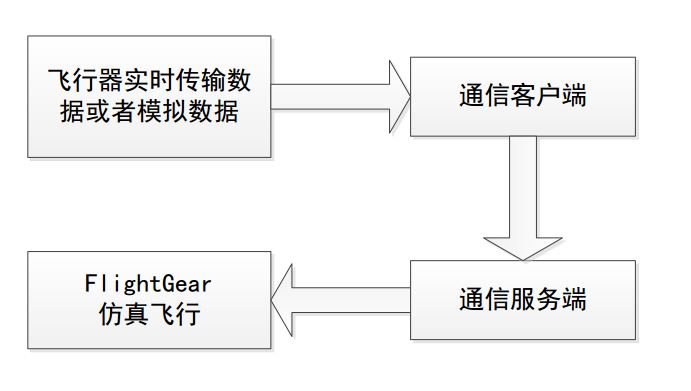
\includegraphics[width=0.6\textwidth]{f22.jpg}
\caption{通信模块的作用}
\label{fig24}
\end{figure}

为了实现在网络中传输数据,必须使用网络通信协议。TIP/IP协议是当前计算机网络中使用最多的网络通信协议,TCP/IP 的核心部分由网络操作系统的内核实现,应用程序通过编程接口来访问TCP/IP\ucite{22}。Socket是介于网络应用层和传输层之间的编程接口,套接字接口提供了访问下层通信协议的大量系统调用函数和相应的数据结构\ucite{23},Socket在通信协议中的地位\ref{fig25}所示。
\begin{figure}[!ht]
\centering
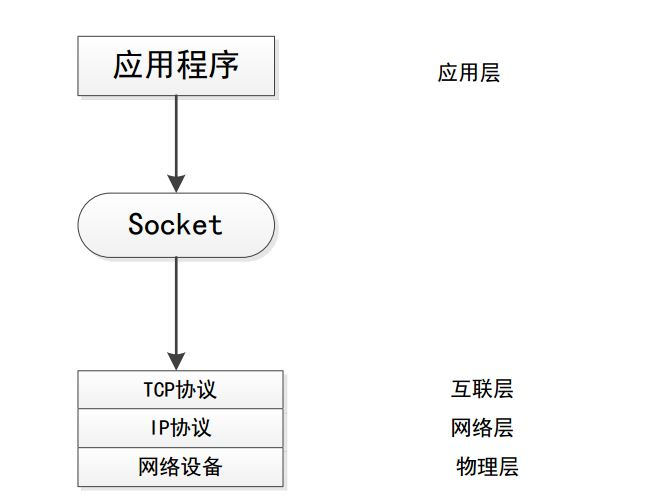
\includegraphics[width=0.6\textwidth]{f23.jpg}
\caption{Socket套接字在TCP/IP通信模型中的地位}
\label{fig25}
\end{figure}

TCP/IP协议的体系结构如图\ref{fig26}所示\ucite{24},其中网络层有两种通信协议TCP和UDP:
 \begin{figure}[!ht]
\centering
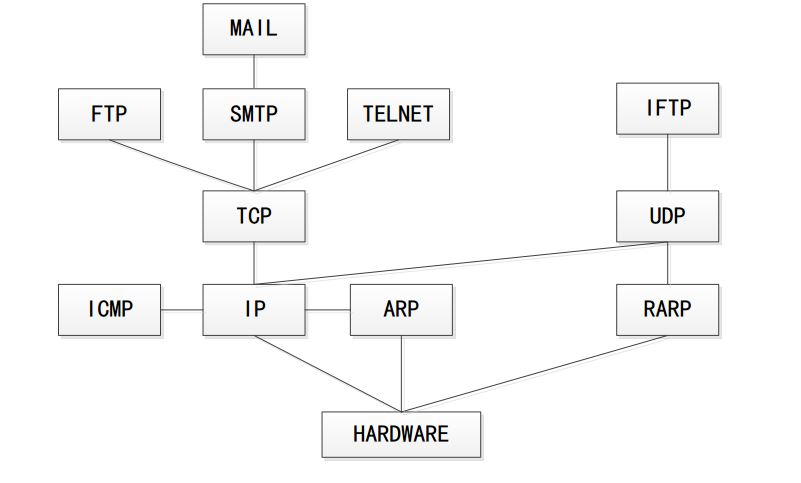
\includegraphics[width=0.6\textwidth]{f24.jpg}
\caption{TCP/IP协议框架}
\label{fig26}
\end{figure}

FlightGear支持使用TCP和UDP两种传输协议进行通信,出于以下几点考虑,本文使用基于数据报套接字的UDP协议开发通信模块:
\begin{itemize}
  \item 行模拟对实时性要求较高,UDP方式不用建立连接通道,不对数据进行校验,传输速率较快,能最大程度的保证飞行模拟的实时性;
  \item 飞行模拟在画面渲染和模拟数据的传输方面对系统资源的开销都很大,UDP方式没有TCP方式对数据质量的控制功能,能降低系统对硬件的要求,最大程度的保证仿真效果;
  \item 飞行模拟对数据的可靠行要求不是非常高,由于前后帧的模拟数据相差很小,丢失一帧甚至几帧的数据不会对模拟结果产生较大影响,因此虽然UDP方式不保证数据无差错,但是使用UDP方式的差错率是可以容忍的。

\end{itemize}

通信模块分为客户端和服务器端,客户端和服务器端可以部署于同一台机器,也可以部署到不同的机器上。在网络中进行通信至少需要一对套接字,其中一个运行于客户端,称之为ClientSocket;另一个运行于服务器端,称之为ServerSocket\ucite{26,27}。本系统使用UDP传输协议实现数据传输的流程图\ref{fig27}。
 \begin{figure}[!ht]
\centering
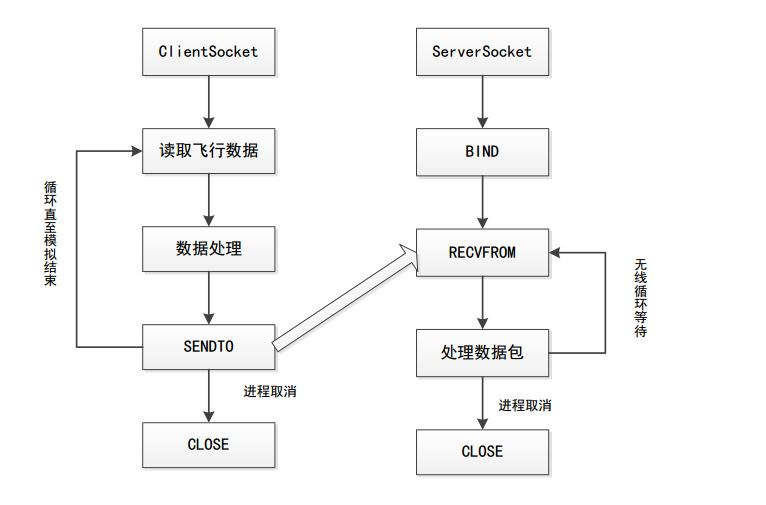
\includegraphics[width=0.8\textwidth]{f25.jpg}
\caption{UDP协议下的客户端与服务端通信流程}
\label{fig27}
\end{figure}
\end{enumerate}
服务器端进程依次进行如下操作:
\begin{itemize}
  \item 调用socket()方法创建一个数据报套接字(SOCK\_DGRAM);
  \item 调用bind()方法将服务器地址绑定在该套接字上;
  \item 调用recvfrom()方法等待客户端发来的数据包,此时程序进入无限循环
等待状态;
  \item 接受客户端传来的数据包,使用该数据包驱动飞行器模型完成相应的
动作;
  \item 继续等待接受客户端的请求;
  \item 服务器端关闭,注销该套接字。
\end{itemize}
客户进程依次进行如下操作:
\begin{itemize}
  \item 调用socket()方法创建一个数据报套接字(SOCK\_DGRAM);
  \item 读取飞行数据,并根据服务器地址向服务器端发送数据报;

数据来源可以是飞行器的实时飞行、动力学模型仿真,也可以是离线的外部数据,或者是FlightGear本身的日志记录文件。本文使用离线外部数据来测试三维可视仿真系统。以C++文件流方式读取外部文件,外部文件来源于joystick的数据读入部分。
\item 数据处理。数据处理主要包括度量单位转换(如弧度与角度转换)、坐标系转换。FlightGear使用测地学坐标系,如果外部数据是基于直角坐标系,则需要进行坐标转换。
\item 继续发送下一条飞行数据;

统通过基于UDP协议的Socket套接字进行发送,发送时间间隔有两种:

一种是指定固定时间间隔进行发送,如20毫秒,即每隔20毫秒发送1次数据,发送时间间隔是固定的;

另一种是根据外部数据的实际生成时间发送,即发送时间间隔不一定是固定的,此方式适合于非匀速变化。
\item 模拟仿真结束,注销该套接字。
\end{itemize}
\section{FlightGear仿真实现}
本节在前面几节的基础上,进行四旋翼的FlightGear飞行仿真的实施步骤及飞行仿真效果。
\subsection{飞行仿真具体实施过程}
\begin{enumerate}
  \item  模型部署

  首先在Linux操作系统中安装FlightGear操作软件,本文的安装路径是“/usr/local/share/FlightGear”。本文选择FlightGear自带的四旋翼模型,如图\ref{fig28}所示。
  \begin{figure}[!ht]
\centering
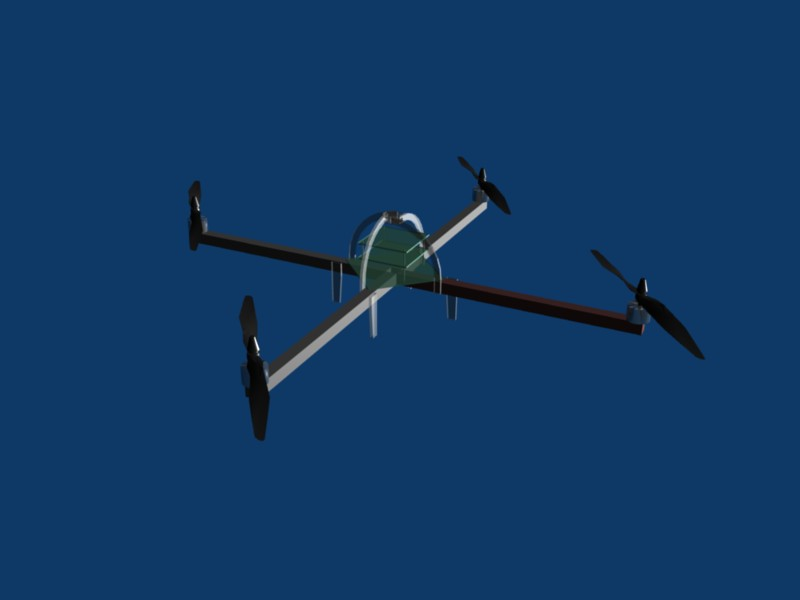
\includegraphics[width=0.4\textwidth]{f31.jpg}
\caption{四旋翼模型}
\label{fig28}
\end{figure}

最后启动 FlightGear 进行调试。在终端窗口内,输入'fgrun',启动 FlightGear 软件,选择“Quadrotor”,选择“next” 设置好飞机场、飞行时间等参数后,点击“run”按钮,如图\ref{fig29}所示。如果顺利进入了图 \ref{fig30}界面,并且伴随螺旋桨轰鸣声,则说明四旋翼无人机飞行模型已经成功配置到了 FlightGear 中,可以使用动力学模型驱动来进行飞行模拟了。
  \begin{figure}[!ht]
\centering
\subfigure[模型选择界面]{
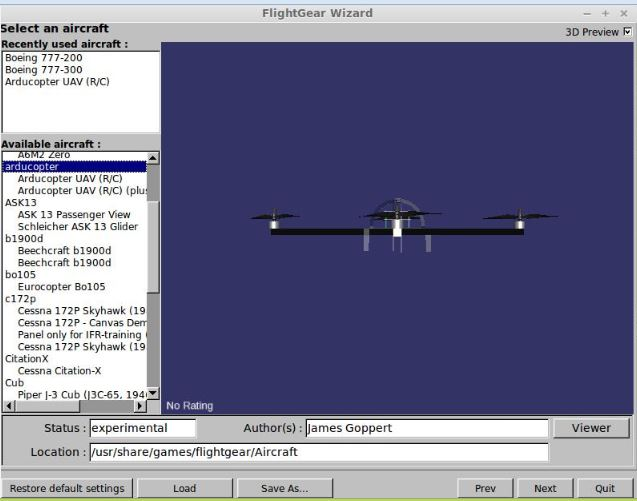
\includegraphics[width=0.45\textwidth]{f32.jpg}\label{f:1}}
\subfigure[机场选择界面]{
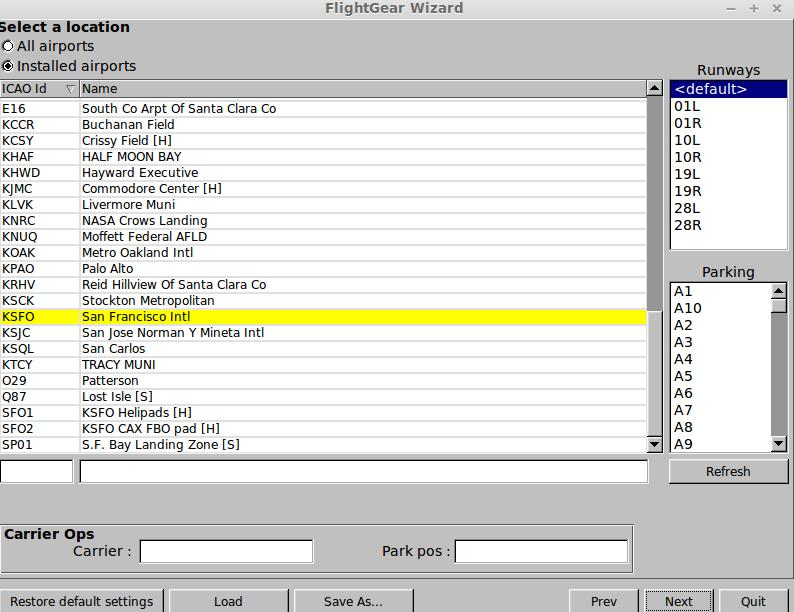
\includegraphics[width=0.45\textwidth]{f27.jpg}\label{f:2}}
\caption{\label{fig29}FlightGear飞行器选择界面}
\end{figure}
\begin{figure}[!ht]
\centering
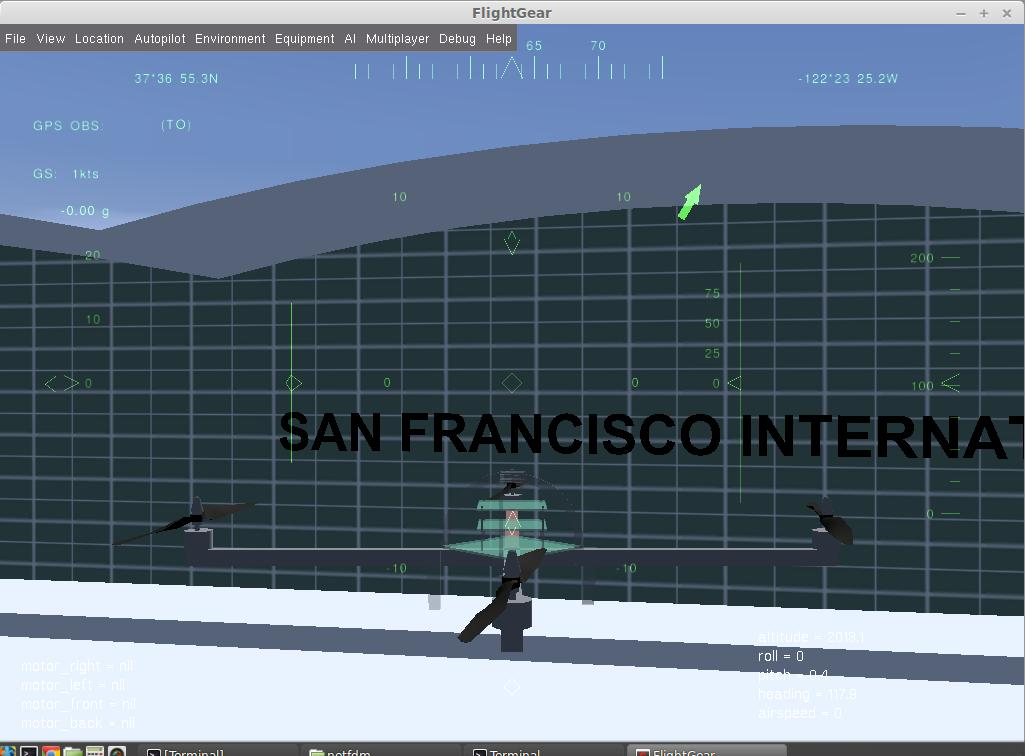
\includegraphics[width=0.8\textwidth]{f40.jpg}
\caption{四旋翼无人机启动界面}
\label{fig30}
\end{figure}
  \item 模型启动

  在完成飞行器模型的部署后,便可以驱动模型进行仿真模拟了。在终端内,输入命令,驱动FlightGear 进行飞行模拟的命令行如下:
\begin{lstlisting}
 fgfs --aircraft=arducopter
      --fdm=network
      --airport=KSFO
      localhost,5501,5502,5503
      --airport=KSFO
 \end{lstlisting}
 --airport=KSFO : 指 定 仿 真 时 使 用 的 飞 机 场 ID , 该 飞 机 场 必 须 在/FlightGear/Airports下能够找到。

 --aircraft=quadrotor:指定仿真时使用的飞行器模型

 --fdm=network:指定仿真使用的动力学模型,可供选择的有:jsb,  larcsim,yasim,  magic,balloon,  external,  pipe, ada,  null。默认的动力学模型是jsb(JSBSim)。network指通过外部数据驱动程序运行(比如通过网络发送的数据)。

  localhost,5501,5502,5503 开启动力学数据连接协议,向fligtgear传送数据。
\end{enumerate}
\subsection{仿真效果}
\begin{figure}[!hbt]
\centering
\subfigure[滚转运动]{
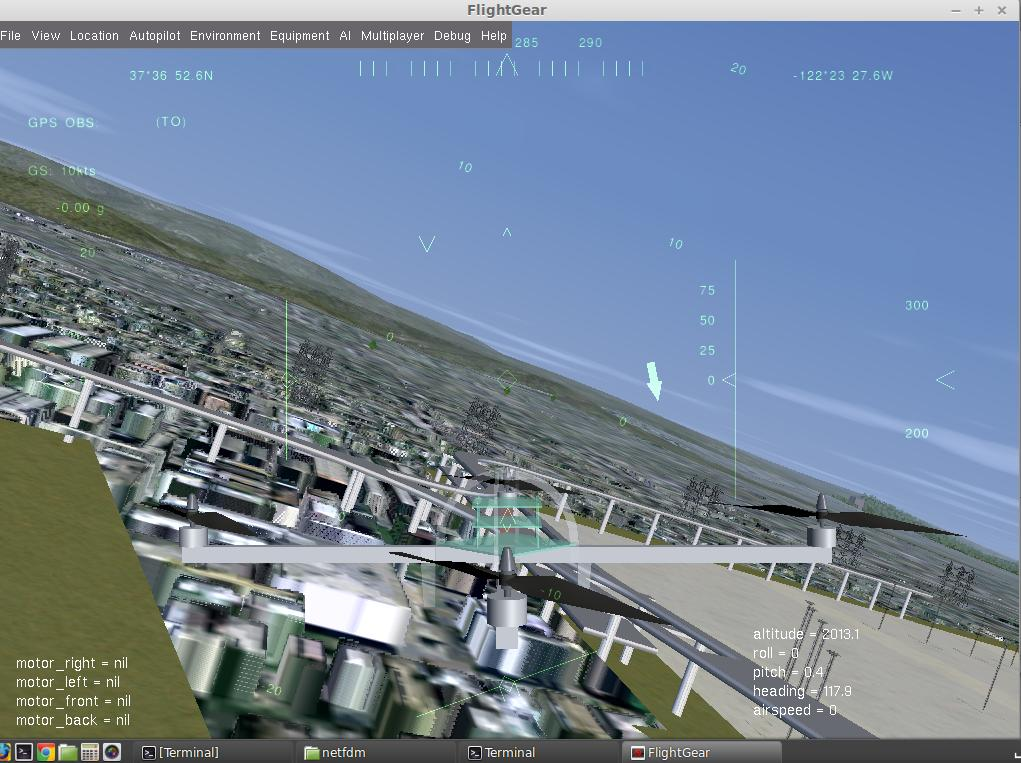
\includegraphics[width=0.4\textwidth]{f41.jpg}\label{f:1}}
\subfigure[俯仰运动]{
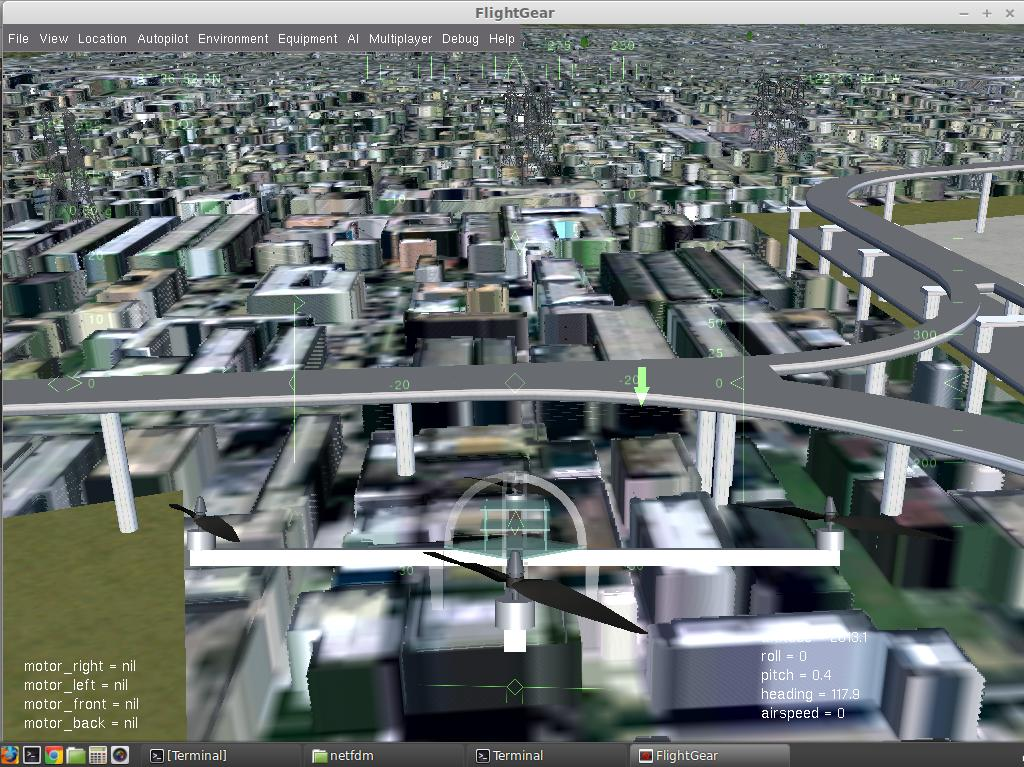
\includegraphics[width=0.4\textwidth]{f42.jpg}\label{f:2}}\\
\subfigure[偏航运动]{
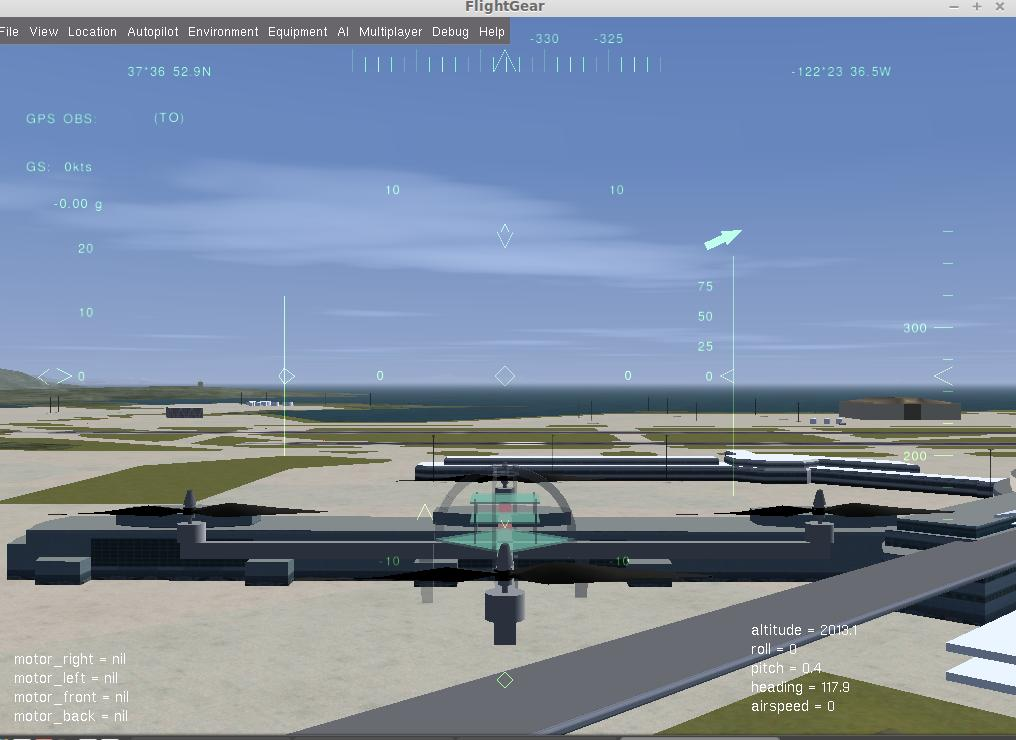
\includegraphics[width=0.4\textwidth]{f43.jpg}\label{f:3}}
\subfigure[空中悬停]{
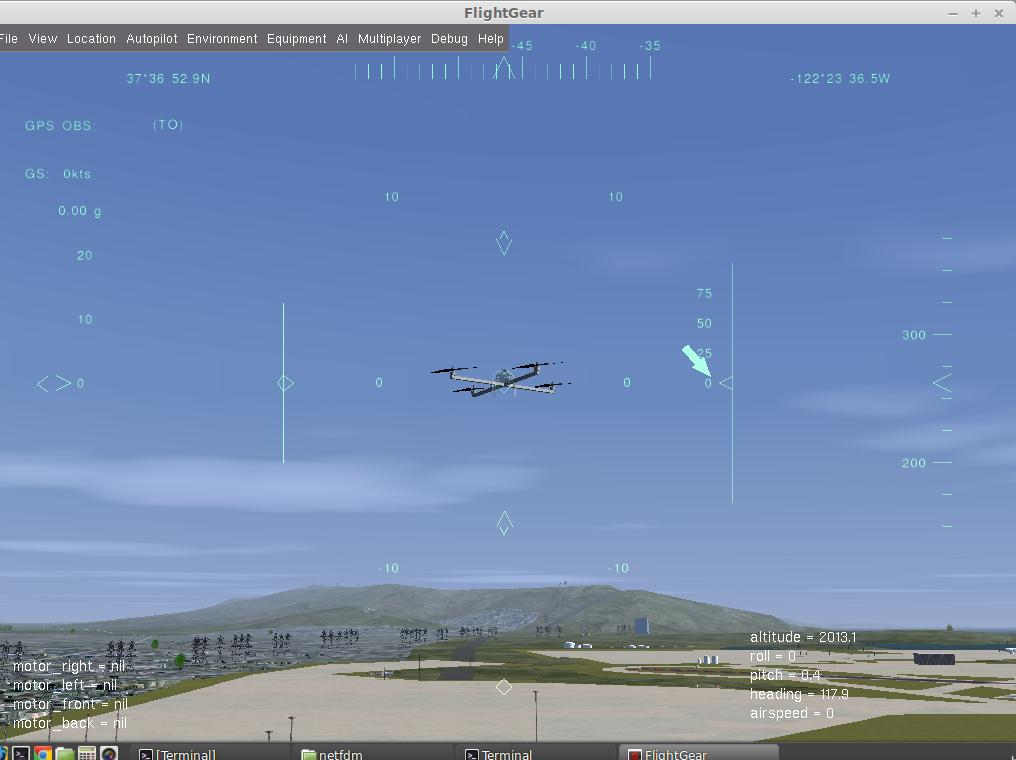
\includegraphics[width=0.4\textwidth]{f44.jpg}\label{f:4}}
\caption{\label{fig31} 四旋翼仿真效果 }
\end{figure}

系统实现了四旋翼无人机飞行的三维可视仿真。将四旋翼无人机的飞行参数(六自由度数据),通过通信模块传递给FlightGear,在飞行参数的驱动下,四旋翼无人机模型在显示屏上可以模拟飞行器起飞、飞行、降落等各种飞行场景,画面连续,可控制播放,可变视角观察(键盘ctrl+V命令),并可进行飞行数据记录与视景回放,达到了设计的预期效果,满足了仿真要求,如图\ref{fig31}所示。